
%(BEGIN_QUESTION)
% Copyright 2011, Tony R. Kuphaldt, released under the Creative Commons Attribution License (v 1.0)
% This means you may do almost anything with this work of mine, so long as you give me proper credit

An Allen-Bradley MicroLogix 1100 PLC senses a 4-20 mA analog signal from a temperature transmitter using an analog input module (model IF2OF2).  At the lower end of signal scale (100 degrees Fahrehneit = 4 mA DC signal), the input register value in the PLC (the analog-to-digital converter's ``count'' value) is 6240.  At the high end of signal scale (800 degrees Fahrenheit = 20 mA DC signal), the input register value in the PLC is 31200:

$$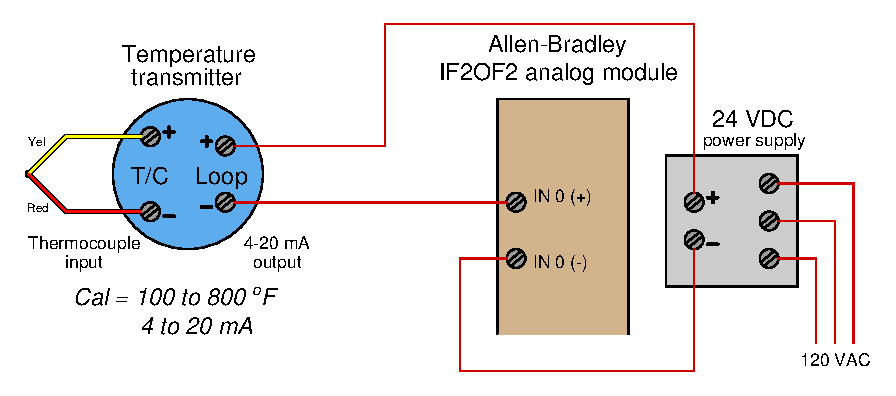
\includegraphics[width=15.5cm]{i03839x01.eps}$$

A {\it scale} (SCL) instruction in the PLC's program is used to convert this raw analog-to-digital ``count'' value into units of degrees Fahrenheit in the PLC, storing the result in register {\tt N7:2} as an integer number:

$$\includegraphics[width=15.5cm]{i03839x02.eps}$$

Examine the parameters entered into this SCL instruction, and then calculate the actual integer value written to {\tt N7:2} at a temperature of 100 degrees F (4 mA signal) and the actual integer value written to {\tt N7:2} at 800 degrees F (20 mA signal).  The results will {\it not} be exact due to rounding of the Rate and Offset parameters.

\vskip 20pt \vbox{\hrule \hbox{\strut \vrule{} {\bf Suggestions for Socratic discussion} \vrule} \hrule}

\begin{itemize}
\item{} The particular scaling chosen here is not the best for a realistic application, using an integer number to represent a temperature between 100 and 800 degrees with a resolution of $\pm$ 1 degree.  Explain how we could represent a temperature range of 100.0 to 800.0 degrees instead.
\item{} For those who have studied thermocouple types, identify the type of thermocouple used in this system.
\item{} Identify the circumstance(s) under which the scale instruction ({\tt SCL}) will generate an {\it overflow} condition in an Allen-Bradley PLC.
\end{itemize}

\underbar{file i03839}
%(END_QUESTION)





%(BEGIN_ANSWER)

At 100 deg F, {\tt N7:2} = 100 {\it (rounded up from 99.72)}

\vskip 10pt

At 800 deg F, {\tt N7:2} = 799 {\it (rounded up from 798.6)}

%(END_ANSWER)





%(BEGIN_NOTES)

The SCL instruction's operation is described in the instruction set manual for the MicroLogix 1100 PLC.  It executes the following mathematical expression:

$$\hbox{Scaled value} = {\hbox{Rate} \times \hbox{Value} \over 10000} + \hbox{Offset}$$

\vskip 10pt

At 100 degrees F, the count value will be 6240.  Therefore, the SCL instruction will carry out the following calculation, which it will round to an integer result of 100:

$$\hbox{Scaled value} = {280 \times 6240 \over 10000} + (-75) = 99.72$$

\vskip 10pt

At 800 degrees F, the count value will be 31200.  Therefore, the SCL instruction will carry out the following calculation, which it will round to an integer result of 799:

$$\hbox{Scaled value} = {280 \times 31200 \over 10000} + (-75) = 798.6$$


%INDEX% PLC, ladder logic program analysis and explanation (Allen-Bradley MicroLogix 1100)

%(END_NOTES)


